\documentclass[12pt,a4paper]{report}
\usepackage[utf8]{inputenc}
\usepackage[T1]{fontenc}
\usepackage{amsmath}
\usepackage{amssymb}
\usepackage{graphicx}
\usepackage{xcolor}
\usepackage{listings}
\usepackage{cite}
\usepackage{subcaption}
\usepackage{float}
\usepackage{algpseudocode}
\usepackage{algorithm}
\usepackage{draftwatermark}
\usepackage{pdfpages}


\SetWatermarkText{DRAFT-2}
\SetWatermarkScale{5}

\author{Josh Pattman}


\graphicspath{{./plots/}}

\newcommand{\checkme}{\textcolor{blue}{\textbf{\emph{VALIDATE THIS STATEMENT}}}}
\newcommand{\citeme}{\textcolor{green}{\textbf{\emph{CITE THIS STATEMENT}}}}
\newcommand{\todo}[1]{\textcolor{red}{\textbf{\emph{TODO: #1}}}}

%\newcommand{\SL}{SwarmAvg }

\title{SwarmAvg: A Novel Approach to Fully Distributed Machine Learning}

% BACKGROUND STUFF
\usepackage{eso-pic}
\newcommand\BackgroundPic{%
	\put(0,0){%
		\parbox[b][\paperheight]{\paperwidth}{%
			\vfill
			\centering
			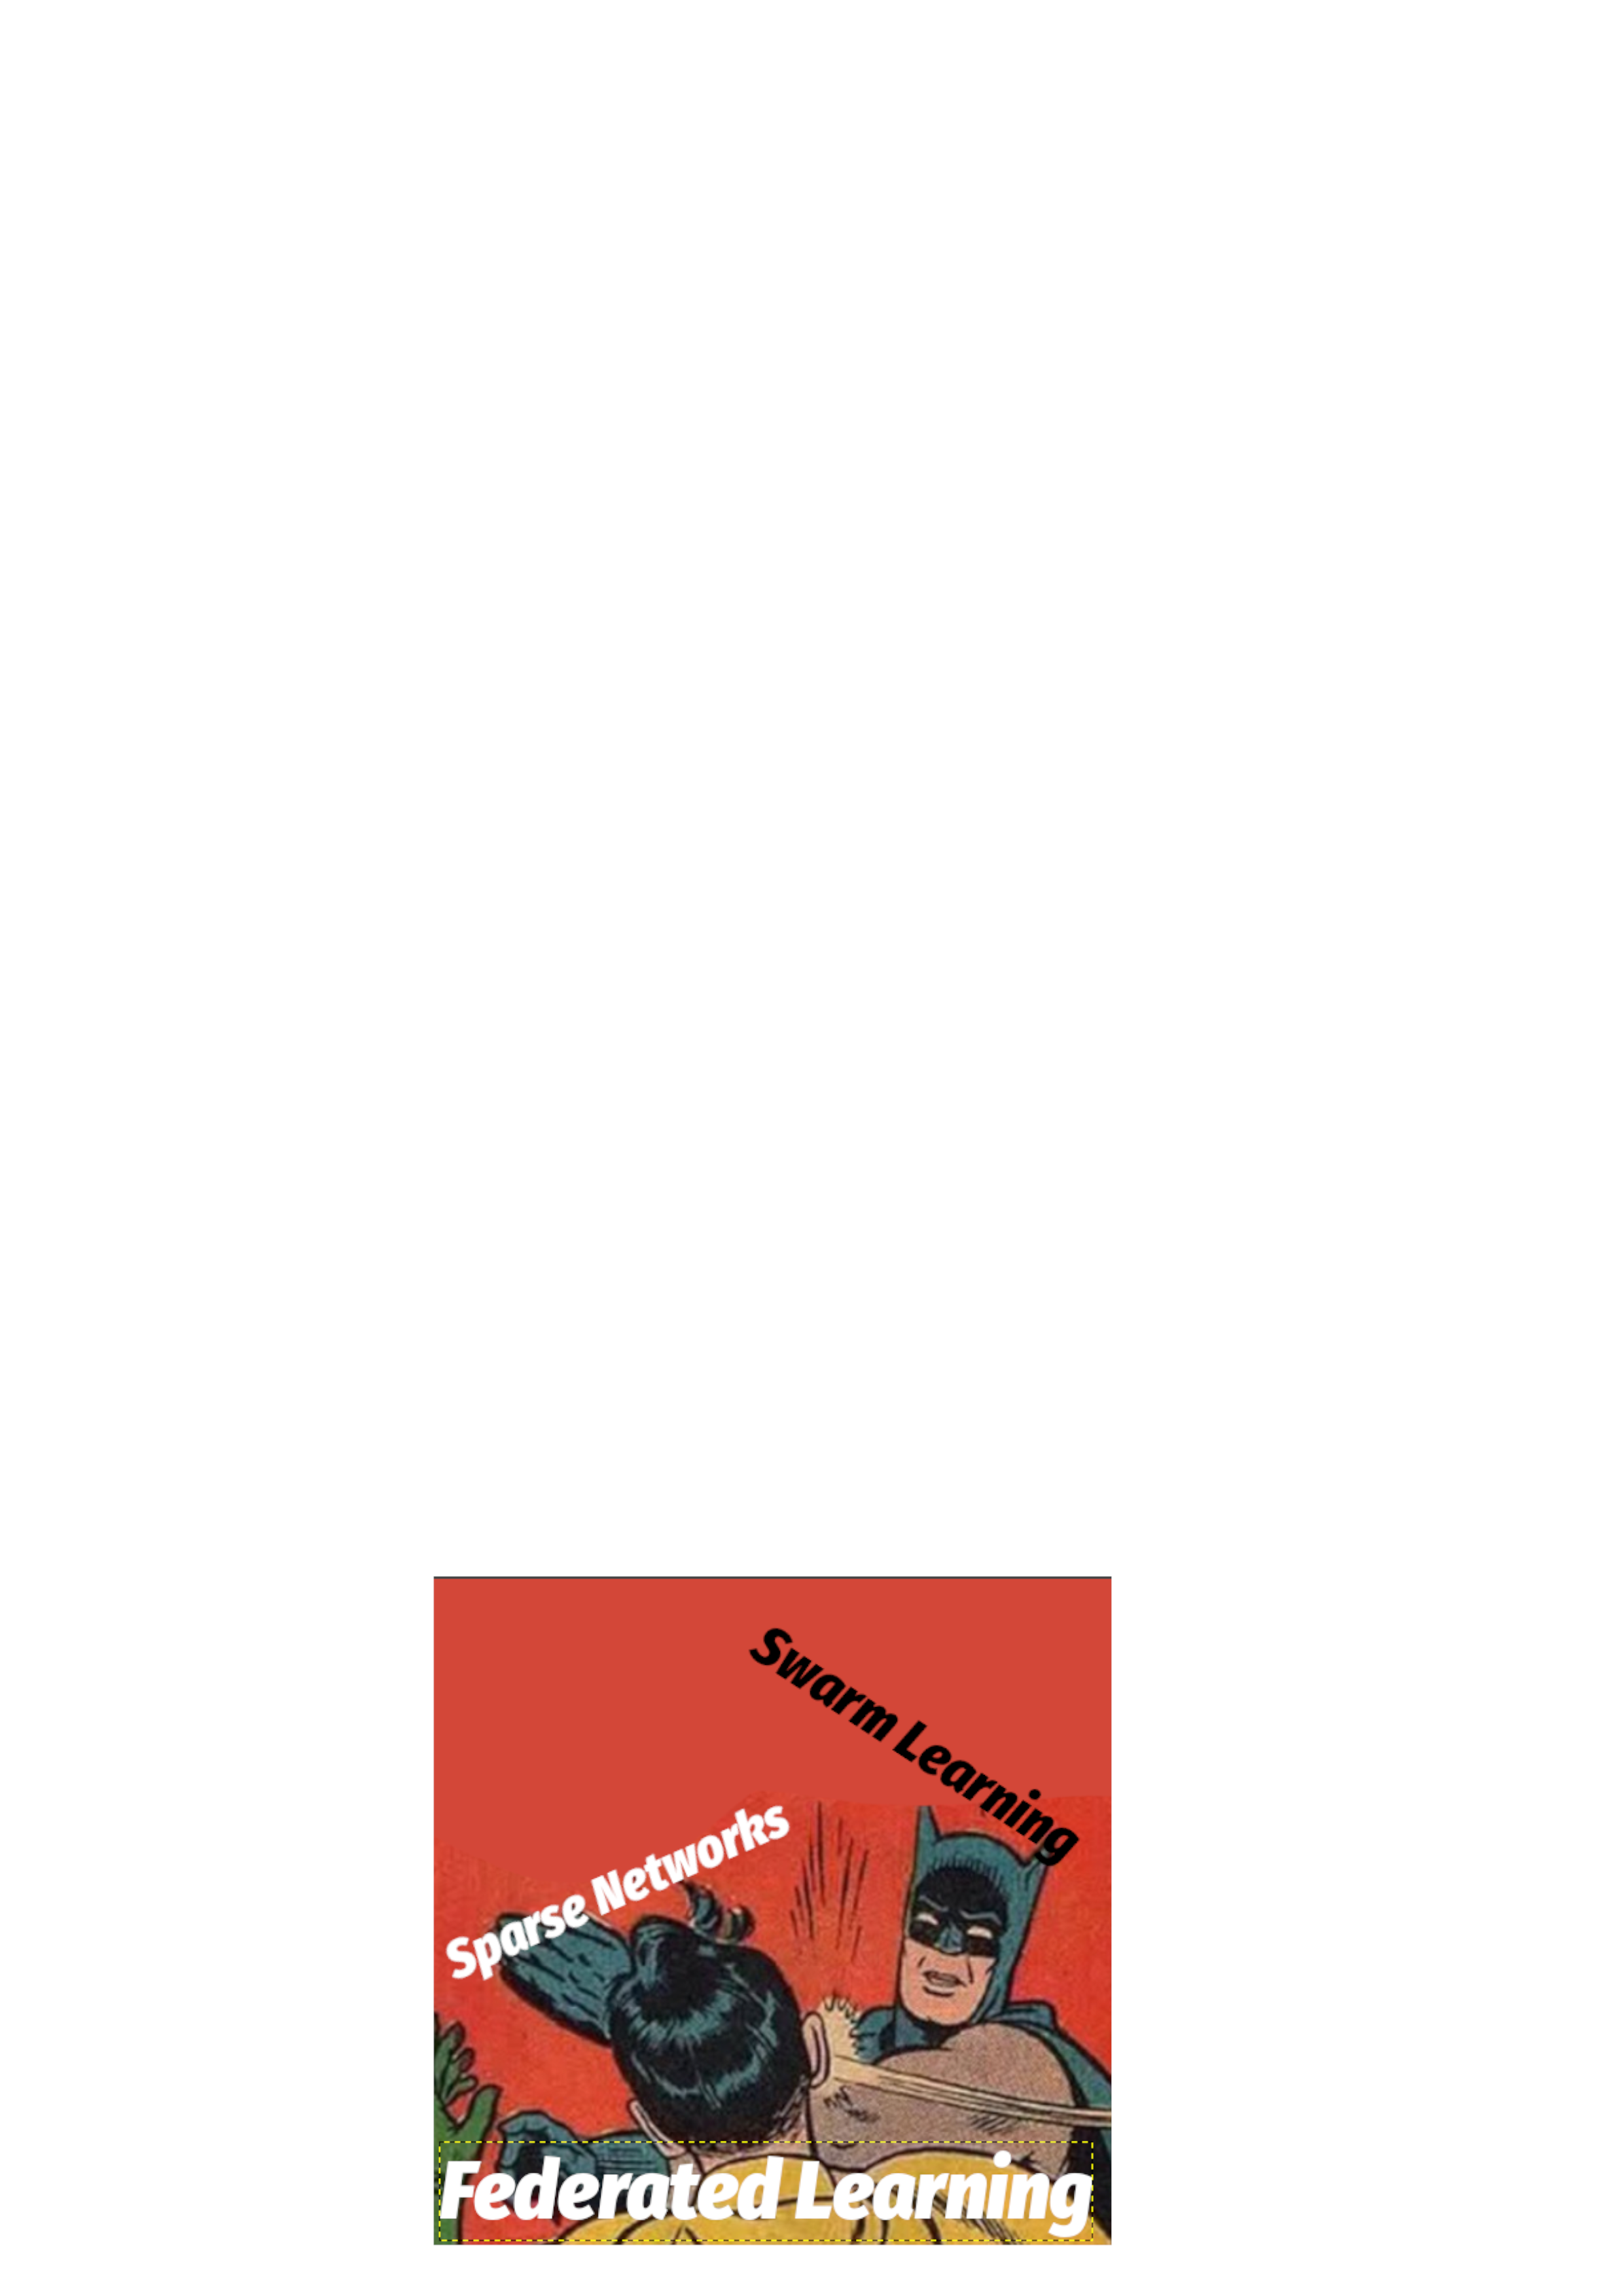
\includegraphics[width=\paperwidth,height=\paperheight,%
			keepaspectratio]{background.png}%
			\vfill
}}}
% END BACKGROUND STUFF

\begin{document}
	% Following line is background stuff
	\AddToShipoutPicture*{\BackgroundPic}
	\maketitle
	
	\chapter*{Abstract}
	\todo{This needs to be slightly reworded and also wordcounted}
	
	Federated learning is a technique that allows a machine learning model to be trained on data distributed across multiple data islands. This approach protects privacy by keeping the data decentralized, meaning that sensitive data does not need to ever be shared. Swarm learning is a similar technique that eliminates the need for a central server, ensuring that not only the data, but also the communication, is completely decentralized. In this paper, a novel swarm learning technique called SwarmAvg is presented which operates without a blockchain. The algorithm is validated against federated learning in various scenarios, and also in some situations where federated learning cannot be applied.
	
	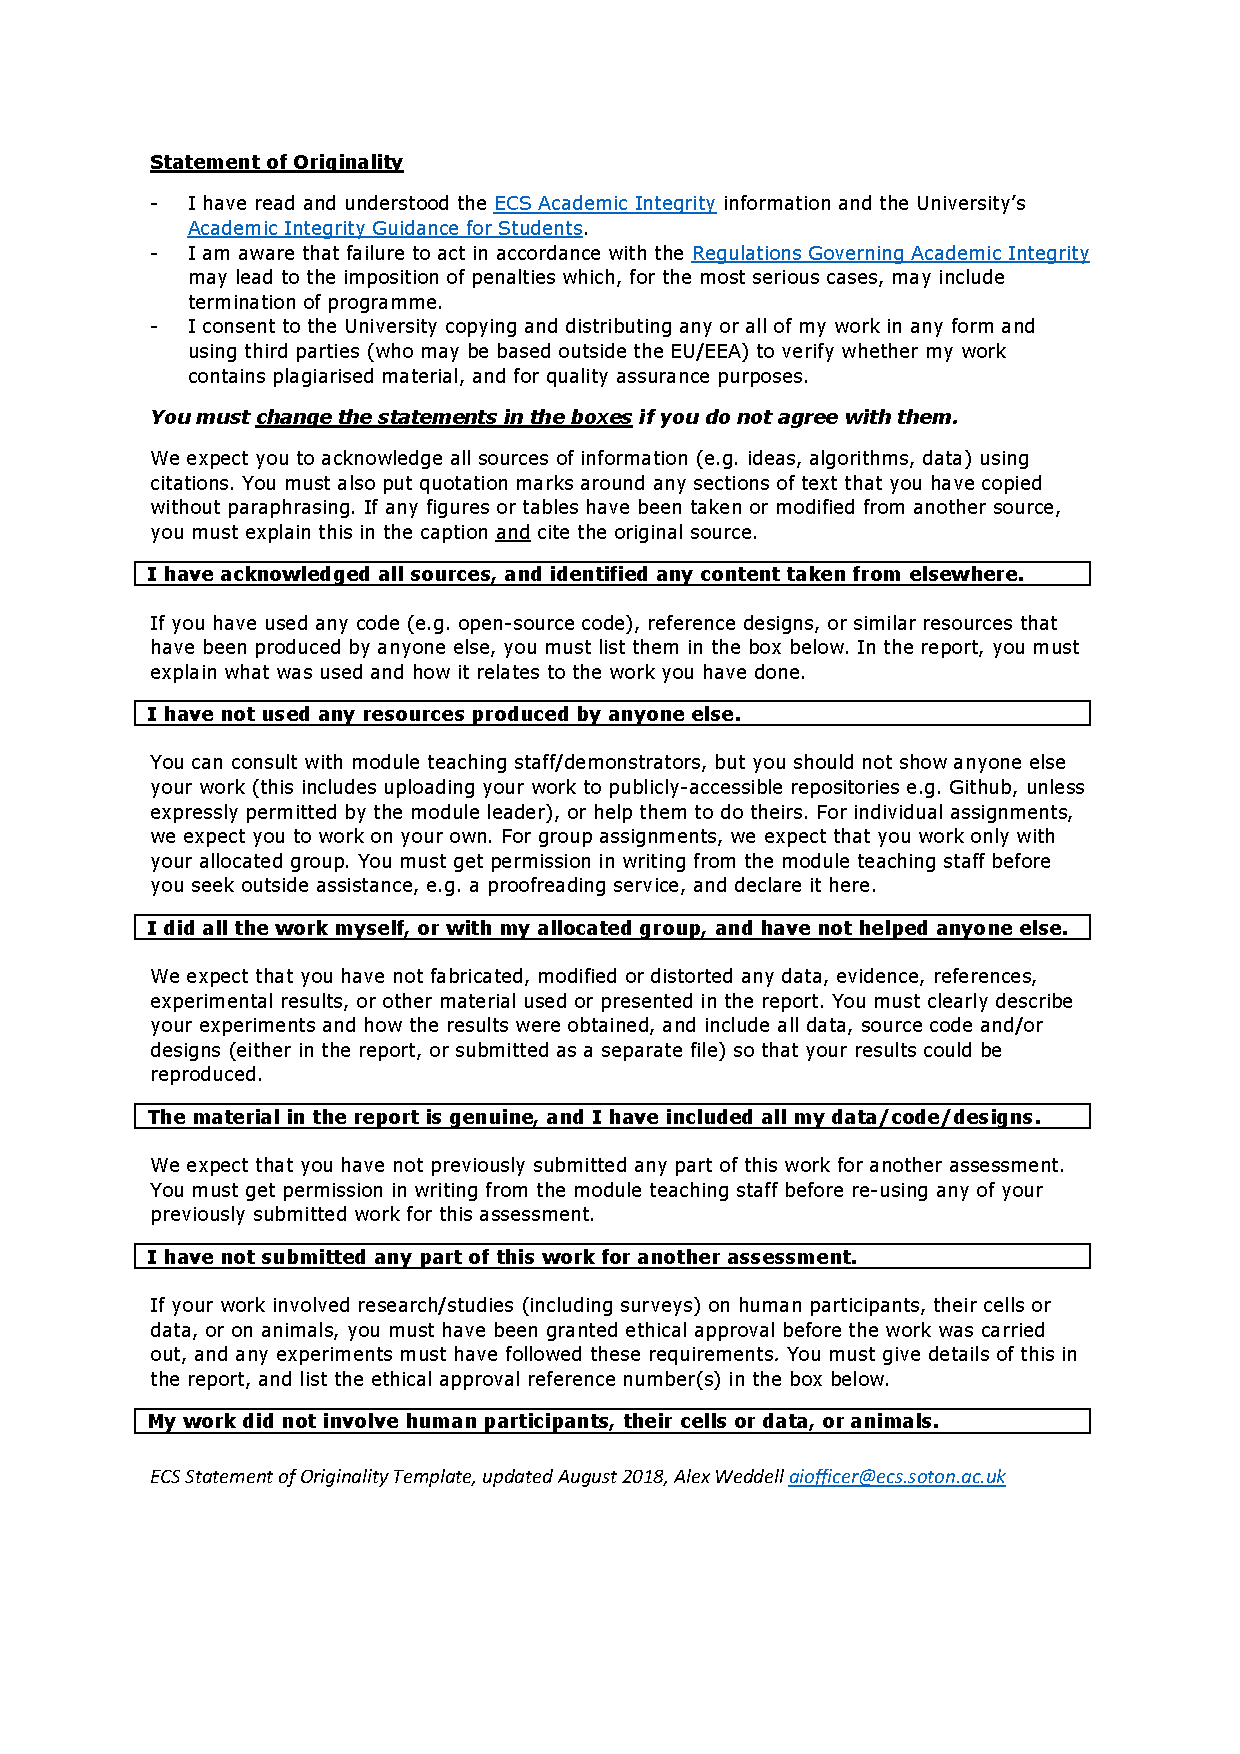
\includepdf[]{soo.pdf}
	
	\tableofcontents

	\chapter{Background} \label{bg}
	\section{Federated Learning}
% Introduce federated learning
Many modern machine learning algorithms require large volumes of diverse data to achieve optimal performance. Real-world data is often distributed among multiple nodes that are unable to share it with each other due to privacy regulations such as GDPR \cite{gdpr}, reducing the amount of data available to train models on and negatively impacting trained performance \cite{data_volume}. Federated Learning (FL) \cite{survey_on_fed_learning} is a technique in machine learning that aims to train a single model using all available data across nodes without requiring any data to be shared among them. \\

% Intro on how fed learning works and different types
There are a multitude of published FL frameworks \cite{fed_table_survey}, each with different merits and drawbacks for certain use cases. Federated Averaging (FedAvg) \cite{fed_learning} is a commonly used yet simple framework, which splits training into iterations where three steps take place:
\begin{enumerate}
	\item A copy of the current model is sent to each node from the central server
	\item Each node performs some training with their copy of the model and their own private data
	\item The trained models from each node are sent back to the server to aggregate into the new server model
\end{enumerate}
The server model improves over time, and after a certain number of steps, the training is complete and the server model is the final output. \\

% Specify why federated learning is better than conventional learning
As it does not require data to be shared between nodes, FL is naturally beneficial for privacy sensitive tasks compared to conventional machine learning where the data is aggregated in a central location \citeme. Additionally, as FL performs training on multiple nodes in parallel, it can make better use of available training resources in situations where processing power is distributed among multiple nodes \citeme.

% federate distributed
One branch of FL is distributed federated learning (DFL). This algorithm works in a very similar fashion to FL, but replaces the central server with an elected leader in a network of nodes \cite{leaderelec_car}. DFL has been shown to increase fault tolerance and security over FL.


\section{Swarm Learning}
% Introduce swarm learning
Swarm learning (SL) is a subcategory of FL which operates in a completely distributed and decentralised manner. SL enables the collaboration of nodes to learn a shared global model, however in contrast to FL, a central server is never used. SL also does not use leader election, so all nodes on the network are given the same importance.

In SL, the model on which new training is performed is known as the global model. However, unlike FL where the global model is stored in a central location, the global model in SL does not materially exist, but is instead a concept which is agreed upon by the nodes in the network.

\begin{figure}[h]
	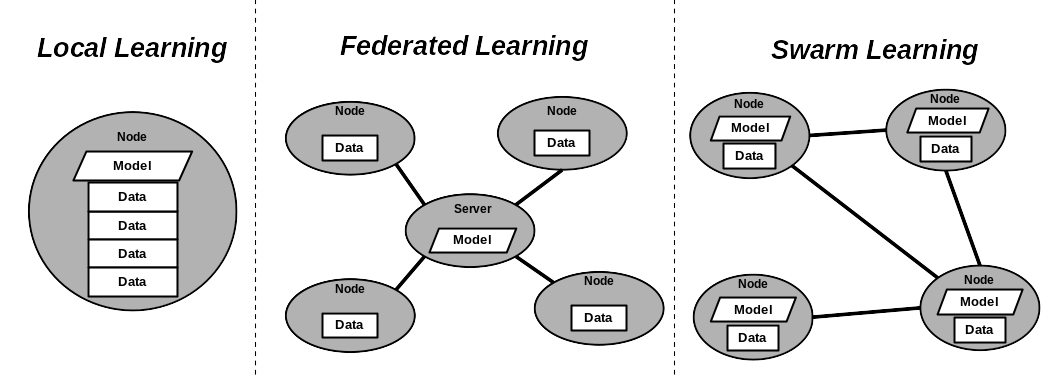
\includegraphics[width=\linewidth]{fedvsswarm}
	\caption{Diagram of different learning algorithms. Each \emph{Node} indicates a single training machine, and each line denotes a connection between two machines, along which the model can be shared. In the swarm learning diagram, the dashed lines show that each local model is an approximation of the global model.} \label{fig_learning}
\end{figure}

One method of SL uses a blockchain to store the global model, enabling the nodes to come to consensus \cite{swarm_learning}. In this version of SL, training is performed by repeating the following steps:
\begin{enumerate}
	\item A node obtains a copy of the global model from the blockchain.
	\item The node performs some training with their copy of the model and their own private data.
	\item The updated model is merged with the latest blockchain model and sent back to the blockchain for other nodes to use.
\end{enumerate}

% Specify why swarm learning is better than conventional learning or federated learning
SL exhibits many of the same benefits of FL over conventional learning, but it also improves upon FL in some aspects. As is often the case when comparing decentralised algorithms to their centralised counterparts \cite{swarm_resil}, the absence of a central server makes SL more resilient to failures than centralized FL approaches such as FedAvg. The lack of a leader election protocol also means that SL may be better suited to tasks where networks of nodes are sparsely connected, as leader election in dynamic networks is a complex problem and can add large amounts of overhead \cite{leaderelection}. Additionally, the removal of the need for a server in SL reduces the likelihood of performance bottlenecks due to network speed constraints for very large swarms.

\section{Blockchain}
\todo{Write this out}

% Breif intro of what a blockcahin is
Blockchain is ... \cite{blockchain_review}

% Disadvantages of using blockchain
%% Scalability
Blockchain has problems with scalability \cite{blockchain_scale}.

%% High transaction cost
Blockchain is inefficient and slow \cite{blockchain_scale}.

	\chapter{Problem and Goals}
	\section{Problem}
In machine learning, there exists some issues that arise from trying to use conventional techniques in the real world.

\subsection{Privacy}
It is common for data to be spread across multiple locations, referred to as data islands. Traditionally, all of this data would be consolidated into a single centralized server to facilitate the process of machine learning. However, it may not be possible to do so, given the potential conflict with privacy legislation. This leaves two options to the data scientist who is looking to train a model: either a single model per data island, likely with inferior performance, or use an algorithm that would allow the different data islands to collaborate and collectively train a model.

Consider this scenario where many different hospitals wish to train a model to detect an illness in a patient. However, due to the obligation to maintain patient confidentiality, the medical data of patients cannot be shared with any of the other hospitals. This means that, despite likely having superior performance, a model trained on all data across all hospitals is not feasible, as a consequence patients would not have the highest quality medical care possible.

\subsection{Performance}
In general, it has been observed that larger machine learning models coupled with more data typically lead to better performance. However, the use of conventional approaches for training these large models necessitates the requirement of a powerful computer. Most entities, however, do not have access to such a computer. Nevertheless, they may have access to multiple, lower-power computers. For instance, during non-working hours, a company may have hundreds of computers in its offices that are not being used, thus providing a pool of unused processing power.

\section{Goals}

\subsection{Design an Novel Algorithm for Swarm Learning}
In this project, the primary aim is to design a novel SL algorithm. This algorithm should be based on FedAvg and \emph{Swarm Learning}. However, the algorithm should be fully decentralised, and it should operate without a blockchain. The decision to not use a blockchain was made due to the disadvantages stated in Section \ref{bg:bc}.

\subsection{Implement the Algorithm}
The primary purpose of the algorithm is to test its viability when compared to other techniques, not to be as efficient as possible for real world usage. Te other important feature of this implementation is that it is easy to replicate by a data scientist who wished to use SL in their next product. For this reason, when implementing the algorithm, an easy-to-understand programming language should be used, and the focus should be on readability rather than absolute performance.

\subsection{Test Performance in Situations Where FedAvg Performs Well}
FedAvg is designed to work in situations where each node has a reliable direct connection to the server. It should be shown that the new algorithm can perform well in similar situations, where each node has many stable connections to other nodes in the network.

\subsection{Test Performance in Situations Where FedAvg Performs Badly}
FedAvg may not be effective when the server has unreliable connections to the nodes, or when nodes are halted. Additionally, if the server stops working, FedAvg is unable to proceed. The goal is to demonstrate that the new algorithm can achieve successful results in scenarios where nodes frequently drop out of the network, thus making it possible to use the algorithm in cases where FedAvg may not be viable.
	
	\chapter{Analysis and Specification of the Solution to the Problem}
	\todo{I don't know what is supposed to go here}
	
	\chapter{Detailed Design}
	\section{Node}
In SL, a node is an agent responsible for facilitating the improvement of the global model. The global model is an abstract concept representing the consensus of all nodes in the network. In the proposed version of SL, referred to as \SL, each node maintains its own model, known as the local model, which is an approximation of the global model. However, in \SL, the consensus algorithm used is repeated averaging, not blockchain. This means that at the start of each training step, every node may start with a slightly different model. As training progresses and performance begins to plateau, each node's local model should not only converge towards a minima, but also towards each other. Over time, each nodes local model better approximates the global model, and the global model becomes a better solution to the problem.

Each node in the network possesses a confidential dataset that is not disclosed to any other nodes. In order to train the global model, nodes fit their own local model of their local dataset. In order to maintain consistency between local and global models, a combination procedure is conducted following each round of local training, which involves the integration of neighbouring nodes models into the local model.

The steps in each training loop for \SL are as follows:
\begin{enumerate}
	\item Fit local model to local dataset.
	\item Send local model to all neighbours.
	\item Combine neighbouring models into local model, using one of the methods presented in Section \ref{mcm}.
\end{enumerate}

In addition, each node retains a local cache of the most recent models of its neighbouring nodes. This cache is updated each time a neighbouring node transmits its model to the node in question, instead of being updated on-demand during the combination step. The reasoning behind this decision is elaborated upon in greater detail in Section \ref{reasonforcache}.

\section{Disposal of Blockchain}
\todo{Write this out}
\begin{itemize}
	\item Neural nets are heuristic - they don't need to be exact
	\item Its just overhead
	\item SL may benefit from large networks, which is bad for bc
	\item SL needs fast BC updates, which is hard
\end{itemize}

\section{Training Counter}
A vital aspect of \SL, specifically the combination step, involves evaluating the performance of a local model. The conventional approach would involve testing each model using an independent test set. However, due to the inability to exchange test sets among nodes, this approach is not feasible as it would result in non-comparable scores for each model. In order to circumvent this problem, this paper presents a heuristic metric referred to as the "training counter," which serves as an approximation of the level of training for a network by estimating the number of training steps performed on a given model.

The training counter can be changed in one of two manners. Firstly, the counter is incremented by 1 when the local model is trained on the local dataset, indicating that an additional step of training has been performed. Following the combination step, the training counter is also updated to reflect the combination method that was utilized. For instance, if the neighbouring models were averaged, the training counter would be updated to represent the average of all neighbouring nodes' training counters.

\section{Model Combination Methods} \label{mcm}
The combination step is a crucial component of \SL. During this step, a node merges its local model with those of its neighbours, producing an updated estimate of the global model. This paper presents multiple methods for performing the combination step.

In the below equations, $\mu(x)$ denotes the function $mean(x)$. All models are assumed to be 1-dimensional arrays, meaning that mathematical operations such as add ($+$) and multiply ($*$) can be performed in an element-wise fashion. To achieve this constraint in the context of neural networks, a simple flattening operation is sued on the weight matrices.

\subsection{Averaging}
The most rudimentary approach to combination is to compute the average model between the local model and the models of all neighbouring nodes.
\[ localModel \gets \mu(localModel \cup neighborModels) \]
This technique is utilized in FedAvg, which is the most simplistic form of FL. The benefit of this method is that it necessitates no hyper-parameters, which means that the data scientist needs to do less tuning. However, this attribute can also be viewed as a drawback, as it affords less flexibility in terms of customization for particular tasks.

\subsection{Averaging With Synchronisation Rate}
A more complex approach to combination is to compute the average model of all neighbours, then compute the weighted average between that model and the local model.
\[ localModel \gets (1 - \alpha) * localModel + \alpha * \mu(neighborModels) \]
The synchronisation rate, denoted as $\alpha$, indicates the degree to which each node adjusts its local model to align with the global model. If $\alpha$ is set too low, each node's model in the network will diverge, resulting in each node becoming trapped at a local minima. On the other hand, if $\alpha$ is too high, the progress achieved by a given node will be discarded at each averaging step, which can result in slower learning.

\subsection{Filtering By Training Counter}
A potential modification to the previously mentioned combination algorithms involves filtering based on the training counter. Specifically, a node may only include its neighbour models if they meet the following statement:
\[neighborTrainingCounter + \beta \ge localTrainingCounter \]
The training offset $\beta$ is the amount the training counter of a neighbour can be behind the local training counter before it is ignored.

A compelling reason to allow training counter filtering is the increased fault tolerance. Consider the situation where node \emph{A} has received many model updates from many nodes, one of which being node \emph{B}. However, node \emph{B} goes offline and no longer is sending model updates. Without training counter filtering, node \emph{A} will continue to combine the outdated node \emph{B} model with it's own for as long as it is training. However, if training counter filtering is enabled, after a number of training steps the outdated model \emph{B} updates will be ignored.

An issue with training counter filtering pertains to the presence of runaway nodes. These nodes possess a substantially higher training counter compared to all other nodes in the network, meaning that when filtering is applied, they are left with no neighbours to utilise in the combination step. Consequently, a runaway node may start to overfit on its own training data, as this is the only data it is exposed to, thereby leading to decreased local performance, as well as potential performance reductions in the rest of the network. To address this problem in \SL, each node must wait until it has obtained at least $\gamma$ viable neighbours prior to performing the combination step. Although this measure prevents individual nodes from becoming runaway nodes, groups of size $\gamma$ still have the potential to become runaway as a unit. Nevertheless, if $\gamma$ is roughly equivalent to the number of neighbours and all neighbours train at a comparable rate, the issue is minimised.

\section{Sparse Network Behaviour}
Given the sparsely connected nature of distributed scenarios, it is often the case that nodes only have direct connections to a small subset of their neighbours. This is a situation where FL struggles, however the author hypothesises that \SL should be able to deal with this situation.

\subsection{Passive Convergence}
An approach to deal with a sparsely connected network is to use the swarm learning algorithm without any modifications. This approach is effective due to the use of averaging as a combination method. When a node tries to update the global model, its changes will propagate through the network slowly, over many training iterations, even to nodes that are not directly connected. This approach has the advantage of requiring no extra data transmission, resulting in significantly less data traffic compared to other methods.

However, this method also has certain theoretical drawbacks. Consider a scenario where the network is comprised of several sparsely connected groups of nodes, where each node in a group is densely connected to other nodes within that group. In this case, it is possible that each group may learn a distinct solution to the problem. This is inefficient because instead of functioning as a cohesive network, there are multiple smaller networks acting somewhat independently of each other, potentially leading to a decrease in overall performance.


\subsection{Relay} \label{relay}
A solution to this could be to relay any received model updates, which means that as long as each node has at least one path to reach all other nodes, the network will behave as a dense network. This approach offers theoretical immunity to changes in network topology, but in practice, the network's performance may still decrease compared to a truly dense network due to slower communication times between non-connected nodes.

The main disadvantage of this approach is the drastic increase in network traffic, which in turn will lead to longer model transfer times. If the swarm learning algorithm is applied to a low power network, such as an IoT network, the increase in network traffic may not be feasible at all. This relay approach can also be applied to federated learning with the same advantages and disadvantages. For these reasons, Relay will not be discussed further.

\section{Complete Algorithm}
\todo{Why this good}
The complete pseudocode algorithm for \SL can be found at Appendix \ref{slalgo}. It has multiple parts which are described below.

The update loop, which can be found at Appendix \ref{slalgo:ul}, is the section of the algorithm which runs continuously during the time which a node is running. It takes care of training and synchronising the local model. The provided code represents what happens in a single update step, meaning that it should be run in a loop that terminates once a stop condition, such as target accuracy, has been reached.

The model received event, which can be found at Appendix \ref{slalgo:mre}, is run on the local node every time a remote node sends the local node a model update. This event takes care of updating the local model cache, to ensure the local node has the most up-to-date information. The model update should contain the model of the remote node and also the remote nodes training counter.

	
	\chapter{Implementation}
	\section{Dataset and Machine Learning Model}
\subsection{Dataset}
Initially, the dataset utilized for experimentation was the MNIST dataset, which encompasses 60000 greyscale 28x28 labelled images of digits from 0 to 9. This dataset was selected for its simplicity, requiring no pre-processing or data cleaning prior to training, and due to its availability as a built-in component of the chosen machine learning framework, Keras.

However, upon implementation it was determined that this dataset was too simple for the application of machine learning, as a single node could reach near peak accuracy after a single epoch, rendering it ill-suited for swarm learning, an algorithm designed to function across multiple training epochs.

To address this issue, the MNIST dataset was replaced with MNIST-fashion, a drop-in replacement dataset containing 10 classes of different items of clothing. MNIST-fashion is known to be more challenging \cite{xiao2017fashionmnist}. To further increase the complexity of the problem, in several experiments each agent was only provided with a small subset of the entire dataset, resulting in less training per epoch, and therefore meaning that an agent would require more epochs to achieve the same performance.

\subsection{Model}
The Keras machine learning framework in Python was utilized to implement the model due to its reputation for being both simple and straightforward. All experiments made use of the same model, which is outlined in Appendix \ref{ap:model} and is a small convolutional neural network. The model was tested on the MNIST fashion dataset and was able to attain an accuracy score of above 90 percent when trained on the entire dataset using local learning; this result is on par with the accuracy reported in the original paper \cite{xiao2017fashionmnist}, making the model suitable for use.


\section{Federated Learning}
FedAvg was chosen for comparison of performance against SwarmAvg. In order to ensure fairness of the comparison, it was necessary to implement FedAvg from scratch using the same language framework as SwarmAvg.
\subsection{Algorithm}
The implemented algorithm worked in the same manner as the algorithm described in the FedAvg paper. However, one modification was made: at the start of each timestep instead of choosing N random nodes to perform training, all nodes were chosen. This means that every available node will perform training at every timestep, which should result in the best possible performance for federated learning, especially give that only 10 nodes could be run at once.

Initially, a REST API was utilised to transfer the model between the server and the client. However, this was deemed unnecessary and was supplanted for two reasons. Firstly, the decision was made to measure performance against epochs trained instead of performance against time, which is discussed in further detail in the results section. Secondly, the REST API approach was much slower than the method chosen to replace it, yet it resulted in the same performance measurements when gauged in terms of epochs trained. As a substitute for the REST API, a system of functions was implemented. When a node sent a model to another node, it simply called a function on that node. This was abstracted away from the main algorithm code, thus meaning that a drop-in REST replacement could b added at a later date. This significantly accelerating training, and enabled a greater number of training runs to be conducted, resulting in more data being collected.

\subsection{Evaluation}
This implementation of federated learning is simple yet effective. Though certain simplifications have been made, they should not interfere with the performance of the model in this scenario. It should only be used for testing performance against epochs trained, not against time taken, as the model transfer layer has been simplified.

\section{Prototype}
It was decided to make an initial, less streamlined, prototype as a proof-of-concept before spending a lot of time creating the final algorithm. This prototype was created to be very modifiable so that changes could easily be made and tested.

\subsection{Algorithm} \label{reasonforcache}
This algorithm was a simplified version of that described in the design section. The primary difference was that when a node performed its synchronisation step, it would request the models from each neighbour instead of utilising its cached versions of their models. This had the consequence of slowing down training, as the synchronisation step could not be completed until all nodes had responded. Furthermore, this algorithm did not incorporate the training counter, leading to the absence of training counter filtering, $\beta$ and $\gamma$.

\subsection{Evaluation}
This step was beneficial for the progression of the project, as it enabled the author to form the ideas detailed in the design process, which were then implemented in the subsequent step. However, due to the abundance of superfluous code, the algorithm was inefficient and performed poorly. For this reason, it was decided not to record the results of this method.

\section{Final Implementation}
In this implementation, the findings of the prototype were taken and built upon. The code was streamlined for the purpose of testing performance. However, the code was still designed to be reusable and easy to read.

\subsection{Algorithm}
The algorithm is as described in the design section. However, there was one discrepancy which needed to be tested: whether to send model updates to neighbours before or after performing the combination step. Both were tested but pushing model updates before combination seemed to be the more effective method when comparing the accuracy. The author hypothesises that this is due to more of the local nodes training progress being preserved, meaning that a local nodes training has more of an affect on its neighbours.

The back end for distributing models was implemented as an interface which abstracts the details of the distribution away from the main algorithm code. For this implementation, the same distribution strategy as the previously implemented FedAvg was used: calling local functions that simulated a web connection.

\subsection{Evaluation}
Overall, this implementation of the proposed swarm learning method is satisfactory. It is efficient, reusable and simple to understand and use. Nevertheless, it is not yet suitable for real world applications, as it lacks any security features and there is limited error handling, being designed for use in a controlled testing environment. However, it would not be challenging to incorporate a backend for this code, allowing for communication over the internet.
	
	\chapter{Testing Strategy and Results}
	\chapter{Testing Strategy and Results}
\section{Strategy for Gathering of Results}
The experiments were conducted through the simulation of a group of nodes on a single computer. The accuracy of each node was evaluated on an unseen test set and subsequently recorded in a file after each training step. All nodes shared the same test set. Below are the specific details of the running of each experiment:
\begin{description}
	\item [Chosen Metric: Accuracy:] The metric chosen for the following experiments was accuracy, due to its comprehensible nature. Despite the fact that an unbalanced dataset presents one of the significant drawbacks of using accuracy, this concern is irrelevant in the case of MNIST-F since it is a balanced dataset, meaning it has the same number of samples in each class. The accuracy of each node is computed after each training step using the test subset of MNIST-F, and none of the nodes are ever provided access to the test set for training.
	
	\item [Number of Simulated Nodes:] The experiments were conducted using 10 nodes, with the exception of the server in cases where FedAvg was employed. The decision of how many nodes to simulate was based on the highest node count attainable without causing inconsistencies and crashes due to resource depletion of the training machine.
	
	\item [Repeated Testing for Noise Reduction:] The training process for each experiment was conducted five times, and the resulting accuracies of every node were recorded. To mitigate the impact of training noise on the performance graphs, the accuracy value for each time step was calculated as the median accuracy across all nodes and runs at that time step. As there were 10 nodes, this resulted in the graphs representing median of 50 nodes.
	
	\item [Configuring the Algorithm:] In each of the following experiments, the algorithm was configured using a specific set of parameters $\alpha \beta \gamma$. These parameters were obtained heuristically by making an initial guess, testing, and then fine-tuning them until a satisfactory outcome was reached. However, it is important to note that an exhaustive investigation into the optimal parameter configuration for a particular type of problem is not within this papers scope, meaning that it is plausible that swarm learning could yield better results with more precisely tuned parameters.
	
	\item [Data Provided to Each Node:] The experiments evaluate the algorithm's performance using three levels of data volume per node. These levels are considerably smaller than the full MNIST-F dataset not only to increase problem difficulty, but also as the algorithm is intended for scenarios where each nodes access to data is restricted. To create a subsection of data for each node, a random sampling with replacement method was used to select the desired number of datapoints. During the initial training phase, each node performs a single sampling of its dataset, after which that nodes data subset remains constant. The three levels of data volume can be seen in Table \ref{epsparams}.
	
	\item [Training Steps and Epochs:] Due to the limited size of the dataset, a single node executes more than one epoch of training in each training step. The number of epochs carried out by a node per training step will be referred to as Epochs per Step (EPS). Empirical testing has indicated that both SL and FL exhibit improved performance with higher EPS, at times surpassing the gains from increasing the number of training steps. Moreover, the utilization of higher EPS was favoured due to its reduced training time, compared to increasing the number of training steps. The three levels of data volume with their respective EPS are shown in table \ref{epsparams}.
	
\end{description}

\begin{table}[H]
	\centering
	\begin{tabular}{l|l}
		Dataset Size & EPS \\ \hline \hline
		1000   & 5  \\ \hline
		100   & 10  \\ \hline
		25  & 20 
	\end{tabular}
	\caption{The different levels of dataset size and EPS that were tested} \label{epsparams}
\end{table}

\section{Scenario 1: Densely Connected Network}
A crucial experiment for evaluating the performance of the SwarmAvg algorithm involves assessing its performance under optimal circumstances, specifically within a network of nodes wherein each node is directly connected to every other node. In FedAvg, the analogous topology involves direct connections between each node and the server. This comparison is significant as it facilitates a direct evaluation of the SwarmAvg and FedAvg algorithms under their respective ideal conditions.

\subsection{Dense Network Results}
The following are the results obtained from the execution of the training script. Each graph displays the data for SwarmAvg in red, and FedAvg in black.

\begin{figure}[H] 
	\center{\textbf{Accuracy by Training Step for 1000 Samples}} \\
	\begin{subfigure}{0.49\textwidth}
		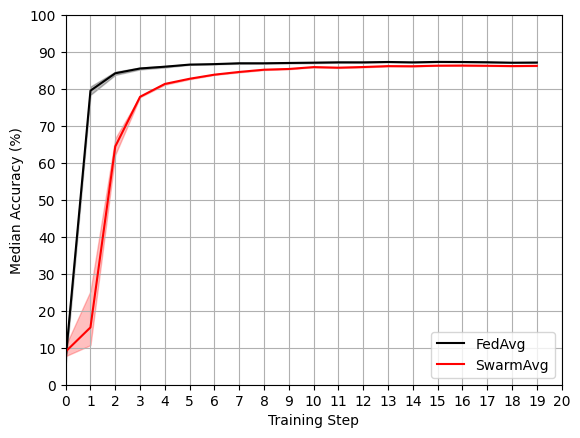
\includegraphics[width=\textwidth]{aeg_dense_1000}
		\caption{Full Graph}
	\end{subfigure}
	\begin{subfigure}{0.49\textwidth}
		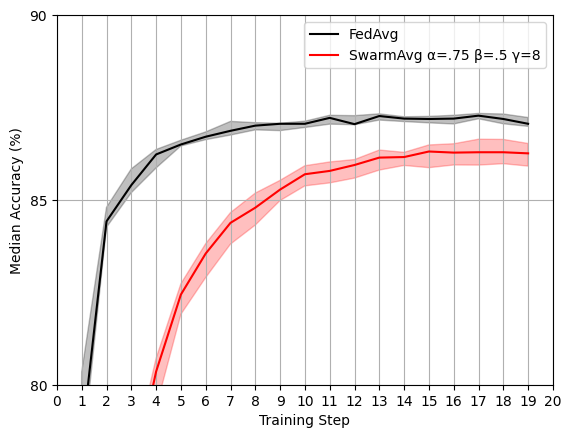
\includegraphics[width=\textwidth]{aeg_dense_1000_z}
		\caption{Zoomed Graph}
	\end{subfigure}
	\caption{Median accuracy by training step across 5 repeats. Each node has 1000 random data samples from MNIST-F. The shaded region represents the upper and lower quartile.}
	\label{aeg1}
\end{figure}

The results depicted in Figure \ref{aeg2} demonstrate that the SwarmAvg algorithm exhibits a slower convergence rate compared to FedAvg, trailing by at least 1 epoch for the duration of the test. Despite this, both methods ultimately achieve a similar level of accuracy, with less than a percent difference.

\begin{figure}[H] 
	\center{\textbf{Accuracy by Training Step for 100 Samples}} \\
	\begin{subfigure}{0.49\textwidth}
		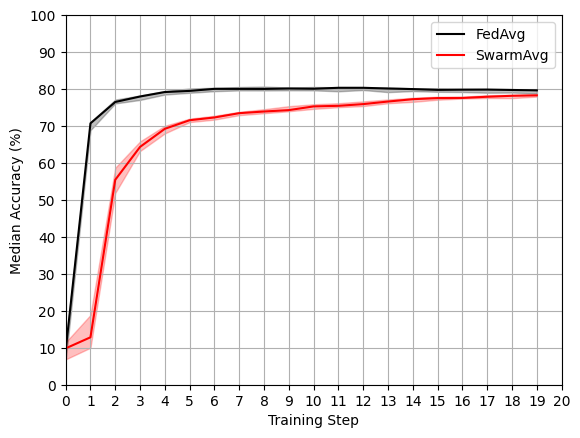
\includegraphics[width=\textwidth]{aeg_dense_100}
		\caption{Full Graph}
	\end{subfigure}
	\begin{subfigure}{0.49\textwidth}
		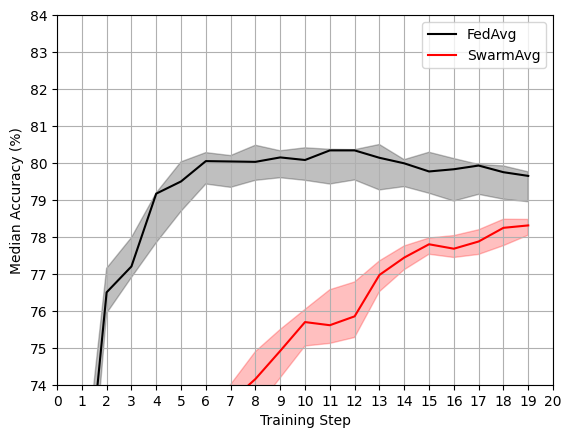
\includegraphics[width=\textwidth]{aeg_dense_100_z}
		\caption{Zoomed Graph}
	\end{subfigure}
	\caption{Median accuracy by training step across 5 repeats. Each node has 100 random data samples from MNIST-F. The shaded region represents the upper and lower quartile.}
	\label{aeg2}
\end{figure}


\begin{figure}[H] 
	\center{\textbf{Accuracy by Training Step for 25 Samples}} \\
	\begin{subfigure}{0.49\textwidth}
		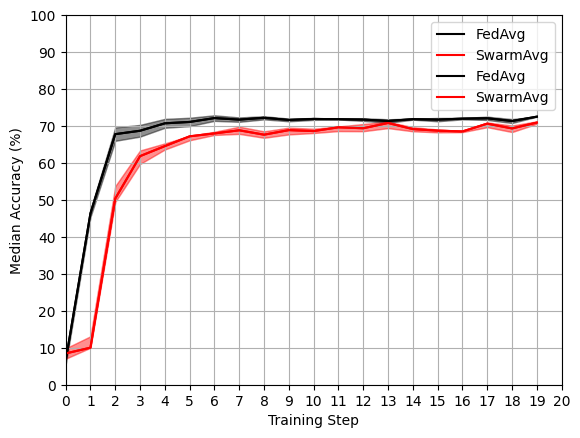
\includegraphics[width=\textwidth]{aeg_dense_25}
		\caption{Full Graph}
	\end{subfigure}
	\begin{subfigure}{0.49\textwidth}
		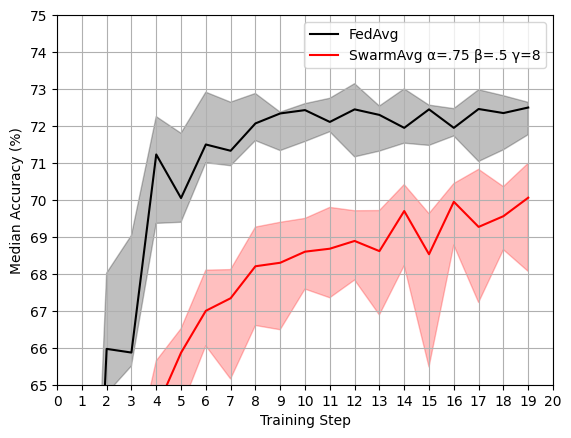
\includegraphics[width=\textwidth]{aeg_dense_25_z}
		\caption{Zoomed Graph}
	\end{subfigure}
	\caption{Median accuracy by training step across 5 repeats. Each node has 25 random data samples from MNIST-F. The shaded region represents the upper and lower quartile.}
	\label{aeg3}
\end{figure}

The trend of SwarmAvg ending with a lower accuracy than FedAvg continues in Figure \ref{aeg3}. Both algorithms also have a much lower accuracy than what they achieved previously, due to the drastic decrease in available data.

Similarly to Figure \ref{aeg2}, Figure \ref{aeg3} shows that SwarmAvg concludes with a lower accuracy than FedAvg. Furthermore, both algorithms exhibit a considerable decline in accuracy when compared to their previous performances with higher volumes of data. \\


The most noticeable impact resulting from reducing the volume of data is the significant decrease in the accuracy of both algorithms, as expected. However, it is also evident that the reduction in data affects SwarmAvg and FedAvg to a similar degree, as both of their peak accuracies stay within a similar range of each other in all tests. The difference in peak accuracy between the two algorithms was quite small, often within a 2 percent margin. \\

One of the prominent challenges associated with SwarmAvg is its slower convergence rate compared to FedAvg, particularly from the outset. SwarmAvg consistently takes a longer time to attain its peak accuracy. This may be attributed to the asynchronous nature of the nodes in SwarmAvg, which implies that some nodes that conduct training before others may have lower accuracy than expected. \\

It is worth noting that in all these evaluations, SwarmAvg has a slightly higher inter-quartile range than FedAvg, indicating that FedAvg is more consistent in terms of accuracy. However, this difference is minor. \\

One interesting feature of both SwarmAvg and FedAvg is that both algorithms seem to be affected by overfitting much less what would be expected. Especially with just 25 data samples per node, the effects of overfitting would usually be far more severe in a single node. However, this does not mean that the algorithms do not overfit, but it may indicate that the process of overfitting for both algorithms is drastically slowed down.

\section{Scenario 2: Sparsely Connected Network}
In reality, it is uncommon for each node to be linked with every other node. To simulate a more realistic scenario, a technique was employed to generate a network of nodes with a specific number of connections. When density is set to 0, the network is minimally linked, meaning that each node has at least one indirect path to every other node, but the minimal number of connections required to accomplish this exist. When density is set to 1, all nodes are connected to one another in a dense fashion. Since this measure may not provide a straightforward indicator of network density, two additional metrics will be provided:  Mean Minimum Hops (MMH) and Mean Connections per Node (MCPN). MMH denotes the mean minimum number of transitions required to get from one node to another in the network. MCPN denotes the average number of connections a given node possess, for a network of 10 nodes. \\

In order to conduct thorough testing on a variety of potential deployment scenarios, several different densities were tested for each count of data. The densities that were tested, along with their corresponding MMH and MCPN, are presented in Table \ref{sparsedensities}.

\begin{table}[H]
	\centering
	\begin{tabular}{l|l|l}
		Density & MMH & MCPN \\ \hline
		1 & 1.0 & 9.0 \\
		0.75    & 1.2 & 7.2  \\
		0.5    & 1.4 & 5.4  \\
		0.25    & 1.7 & 3.6  \\
		0    & 3.0 & 1.8  \\
	\end{tabular}
	\caption{The statistics for different density levels} \label{sparsedensities}
\end{table}

In order to assist the reader with visualizing the various density levels, some sample networks that were generated for each density can be found in Figure \ref{densefig}.

\begin{figure}[H]
	\centering
	\begin{subfigure}[b]{0.3\textwidth}
		\centering
		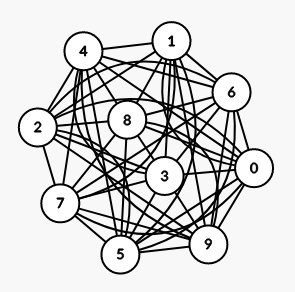
\includegraphics[width=\textwidth]{sparsegraph100}
		\caption{$density=1.0$}
	\end{subfigure}
	\begin{subfigure}[b]{0.3\textwidth}
		\centering
		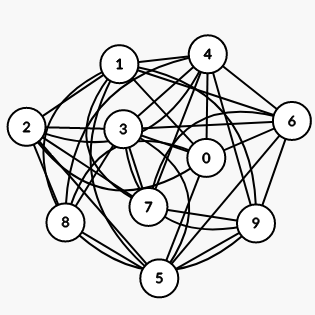
\includegraphics[width=\textwidth]{sparsegraph75}
		\caption{$density=0.75$}
	\end{subfigure}
	\begin{subfigure}[b]{0.3\textwidth}
		\centering
		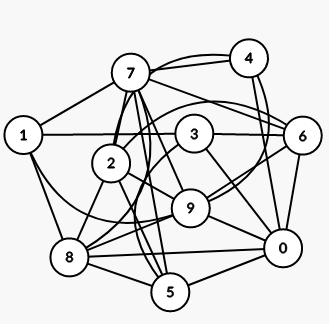
\includegraphics[width=\textwidth]{sparsegraph50}
		\caption{$density=0.5$}
	\end{subfigure}
	\begin{subfigure}[b]{0.3\textwidth}
		\centering
		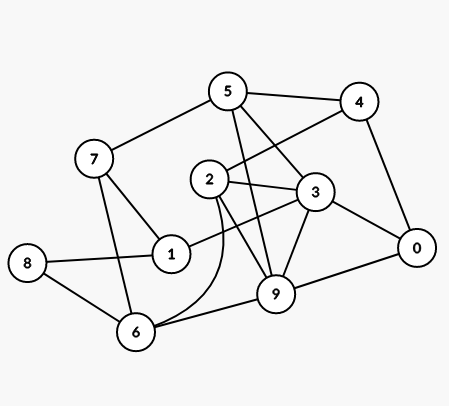
\includegraphics[width=\textwidth]{sparsegraph25}
		\caption{$density=0.25$}
	\end{subfigure}
	\begin{subfigure}[b]{0.3\textwidth}
		\centering
		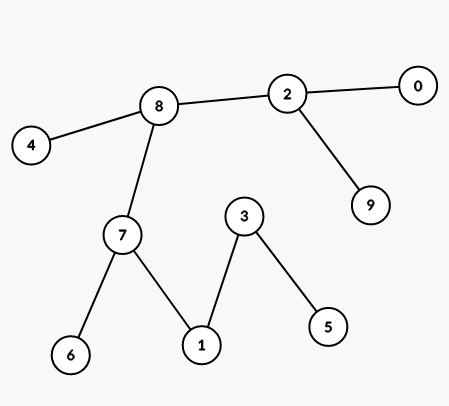
\includegraphics[width=\textwidth]{sparsegraph0}
		\caption{$density=0.0$}
	\end{subfigure}
	\caption{Example networks of nodes generated for each density level, visualised using the tool at \emph{https://csacademy.com/app/graph\_editor}. Each time a simulation is started, a new random network is generated for that simulation. \label{densefig}}
{}\end{figure}


This section does not include any testing of FedAvg. In scenarios where not every node is directly connected to the server node, FedAvg has two potential options: ignore all nodes which are not directly connected, or attempt to relay the model updates through connected nodes. As mentioned in Section \ref{relay}, relaying may not always be the optimal solution. Ignoring nodes is also not a good option, as data is wasted. Therefore, in this test, the decision was made to solely evaluate SwarmAvg.


\subsection{Sparse Network Results}
Below are results obtained from testing. The density of each line on the graph is indicated by the colour, with a green hue representing higher density and a red hue indicating lower density. For all tested densities, the value of $\gamma$ was set to $round_{down}(MCPN) - 1$, which ensures that each node can progress only after waiting for all but one of its neighbours. Notably, failure to reduce $\gamma$ for less dense networks would cause several nodes to wait for a number of neighbours that cannot be achieved. Due to the random nature of the graph generation, there will still be some nodes who have less than $\gamma$ neighbours, but this should be rare and the loop to wait for $\gamma$ neighbours will terminate after a certain number of tries anyway, ensuring that training can progress.

\begin{figure}[H] 
	\center{\textbf{Accuracy by Training Step for 1000 Samples, with Varying Density}} \\
	\begin{subfigure}{0.49\textwidth}
		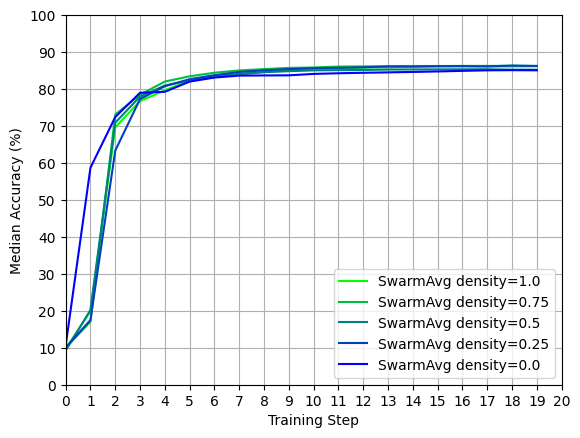
\includegraphics[width=\textwidth]{aeg_sparse_1000}
		\caption{Full Graph}
	\end{subfigure}
	\begin{subfigure}{0.49\textwidth}
		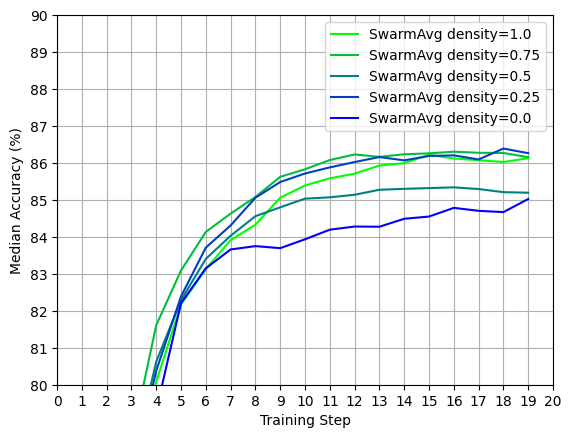
\includegraphics[width=\textwidth]{aeg_sparse_1000_z}
		\caption{Zoomed Graph}
	\end{subfigure}
	\caption{Median accuracy by training step across 5 repeats. Each node has 1000 random data samples from MNIST-F. Quartiles are not shown.}
	\label{aeg4}
\end{figure}

An observation that can be made of Figure \ref{aeg4} is that the different network densities perform very similarly. The final accuracy for all of the tests fell within a 2 percent range,  with the higher densities occupying the higher end. \\

One interesting feature of the Figure \ref{aeg4} is that the lowest density demonstrates faster convergence initially that the other densities. The author hypothesises that this may be due to groups of nodes forming local sub-networks which converge on their own sub-sets of data faster, but more slowly combine into the network as a whole as training progresses.

\begin{figure}[H] 
	\center{\textbf{Accuracy by Training Step for 100 Samples, with Varying Density}} \\
	\begin{subfigure}{0.49\textwidth}
		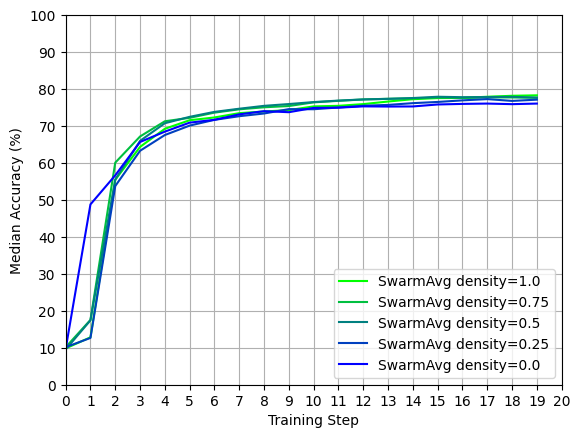
\includegraphics[width=\textwidth]{aeg_sparse_100}
		\caption{Full Graph}
	\end{subfigure}
	\begin{subfigure}{0.49\textwidth}
		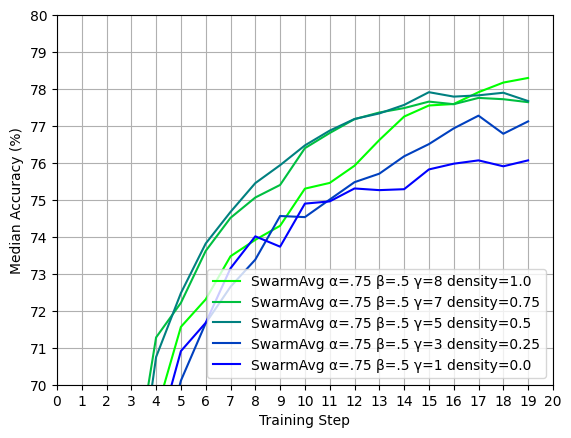
\includegraphics[width=\textwidth]{aeg_sparse_100_z}
		\caption{Zoomed Graph}
	\end{subfigure}
	\caption{Median accuracy by training step across 5 repeats. Each node has 100 random data samples from MNIST-F. Quartiles are not shown.}
	\label{aeg5}
\end{figure}

In Figure \ref{aeg5}, there is a greater spread of final accuracies, about 2.5 percent, than is shown in Figure \ref{aeg4}. The more noticeable feature of Figure \ref{aeg5} is that the final accuracies of all densities are approximately 8 percent lower than their counterparts with more data available in figure \ref{aeg4}.

\begin{figure}[H] 
	\center{\textbf{Accuracy by Training Step for 25 Samples, with Varying Density}} \\
	\begin{subfigure}{0.49\textwidth}
		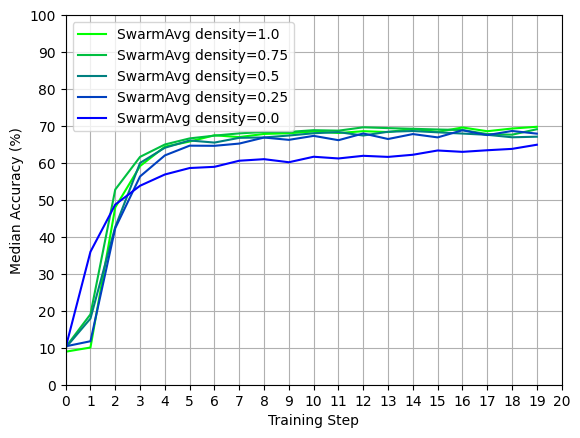
\includegraphics[width=\textwidth]{aeg_sparse_25}
		\caption{Full Graph}
	\end{subfigure}
	\begin{subfigure}{0.49\textwidth}
		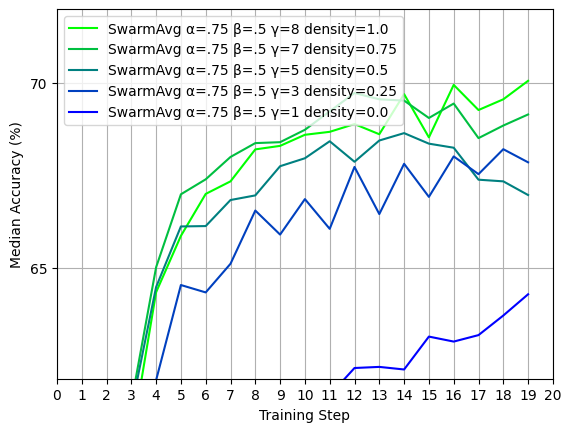
\includegraphics[width=\textwidth]{aeg_sparse_25_z}
		\caption{Zoomed Graph}
	\end{subfigure}
	\caption{Median accuracy by training step across 5 repeats. Each node has 25 random data samples from MNIST-F. Quartiles are not shown.}
	\label{aeg6}
\end{figure}

With 25 data samples, the tests depicted in Figure \ref{aeg6} show a much higher variation in final accuracies than the previous two figures. There is also a much higher degree of noise in this figure than any other, suggesting that training may be much less stable with this small number of data samples to train on.

It should also be noted that the lowest density is still exhibiting the behaviour of outperforming the other densities in the initial steps, however it appears that this effect has become slightly less prominent. \\


Generally, altering the network density of nodes has a small impact on the training of the nodes within the network. Decreasing the density of nodes typically leads to a lower final accuracy. This effect becomes more noticeable as the data volume provided to each node decreases, as demonstrated by the increased variability in training displayed in Figure \ref{aeg6} in comparison to Figures \ref{aeg4} and \ref{aeg5}. \\

The networks possessing a density of 0 attain their optima at a faster rate than those with higher densities. Figure \ref{aeg6} illustrates that the lower densities reach convergence marginally quicker than higher densities, yet are surpassed by the latter towards the end of training.

\section{Scenario 3: Densely Connected Network with Class Restrictions}

Decentralized machine learning algorithms, such as FedAvg and SwarmAvg, commonly involve a scenario where each node possesses a dataset whose distribution does not align with the overall data distribution across all nodes. In order to simulate such a scenario, a situation was created where each node was given access a unique set of three out of ten classes of MNIST-F. The tests in this experiment were conducted in a densely connected network of nodes, thereby allowing the evaluation of FedAvg as well.

\subsection{Dense Network with Class Restrictions Results}

\begin{figure}[H] 
	\center{\textbf{Accuracy by Training Step for 1000 Samples of 3 Classes}} \\
	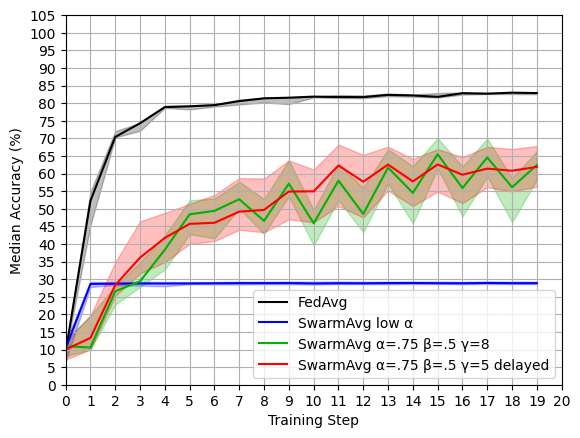
\includegraphics[width=0.49\textwidth]{aeg_unev_1000}
	\caption{Median accuracy by training step across 5 repeats. Each node has 1000 random data samples from MNIST-F. Quartiles are depicted as the shaded area. Each node has access to a unique set of 3 classes out of 10}
	\label{aeg7}
\end{figure}

During the course of the experiment, it was determined that SwarmAvg required some adjustments in order to function properly. One issue was a significant fluctuation in accuracy during the training process, which may have been due in part to the synchronization of nodes in the network. To address this concern, the decision was made to decrease the value of $\gamma$ and introduce a delay in the node start times, in order to desynchronize their training. The chosen delay time was 2 seconds. Figure \ref{aeg7} illustrates these two techniques, with the delayed training and reduced gamma method depicted in red, and the original method depicted in green. Evidently, these adjustments had a positive impact in minimizing the oscillations, although they were not entirely eliminated. \\

While attempting to adjust the parameters, another issue was encountered was divergent training, which occurs when nodes begin to learn completely separate models and start to disregard the models of their neighbours. It was observed that a low value of $\alpha$ was sufficient to cause this problem. When divergent training occurred, the nodes failed to achieve an accuracy level higher than 30 percent, which is expected if a node only trains on three out of the ten available classes. This effect is shown as the blue line of Figure \ref{aeg7}. \\

It is evident that SwarmAvg consistently exhibits a significantly lower level of accuracy compared to FedAvg. Additionally, the inter-quartile range of SwarmAvg is noticeably higher.

\begin{figure}[H] 
	\center{\textbf{Accuracy by Training Step for 100 and 25 Samples, with 3 Classes}} \\
	\begin{subfigure}{0.49\textwidth}
		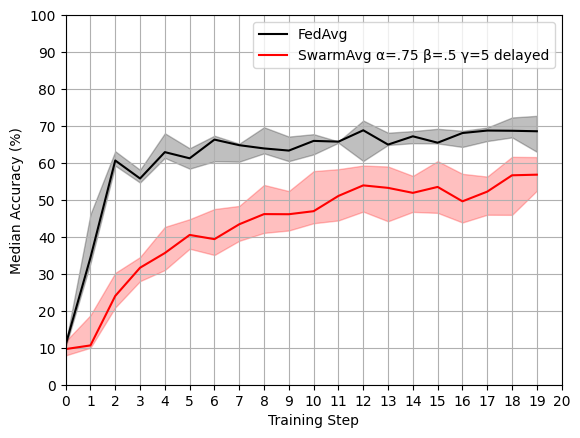
\includegraphics[width=\textwidth]{aeg_unev_100}
		\caption{Samples=100}
	\end{subfigure}
	\begin{subfigure}{0.49\textwidth}
		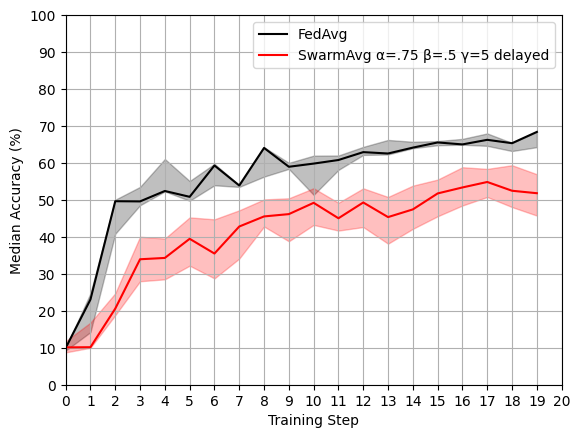
\includegraphics[width=\textwidth]{aeg_unev_25}
		\caption{Samples=25}
	\end{subfigure}
	\caption{Median accuracy by training step across 5 repeats. Quartiles are depicted as the shaded area. Each node has access to a unique set of 3 classes out of 10}
	\label{aeg8}
\end{figure}

When performing training on a lower sample count, as depicted in Figure \ref{aeg8}, the oscillations in SwarmAvg seem to have been drastically reduced when compared to \ref{aeg7}. However, both SwarmAvg and FedAvg have lower accuracies by the end of training than they did with 1000 samples. \\

It is clear that the reduction of data volume per node has a detrimental impact on the performance of SwarmAvg in general. However, in these restricted class tests, this effect is less pronounced compared to previous tests where each node had access to all possible classes. It should be noted that SwarmAvg encounters accuracy oscillations, which can be partially attributed to the synchronized training steps of nodes. Nevertheless, by decreasing the value of $\gamma$ and staggering the startup of nodes, these oscillations can be mitigated. Moreover, reducing the data volume also seems to aid in reducing the effect of these oscillations, possibly implying that nodes are being trained excessively in a single step.

\section{Scenario 4: Sparsely Connected Network with Class Restrictions}
This scenario was designed to test the SwarmAvg algorithm to its limits. It not only involved limiting data to each node, but also limiting the classes each node had access to in the same fashion as Scenario 3, and also constraining the networks to be sparsely connected.

\subsection{Sparse Network with Class Restrictions Results}
\begin{figure}[H] 
	\center{\textbf{Accuracy by Training Step for 1000, 100 and 25 Samples, with 3 Classes and Varying Density}} \\
	\begin{subfigure}{0.49\textwidth}
		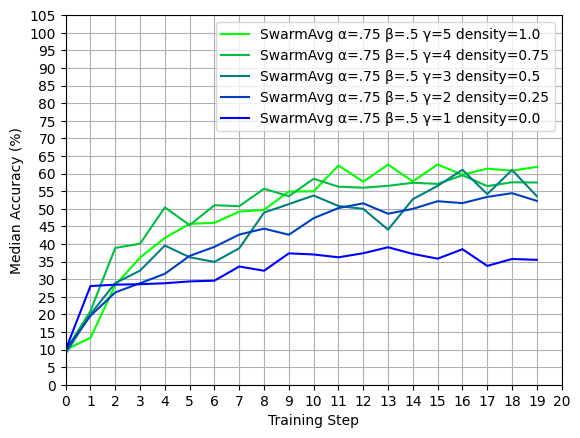
\includegraphics[width=\textwidth]{aeg_sparse_unev_1000}
		\caption{Samples=1000}
	\end{subfigure}
	\begin{subfigure}{0.49\textwidth}
		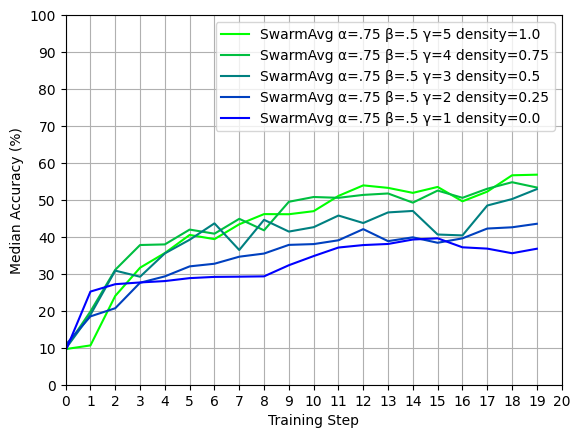
\includegraphics[width=\textwidth]{aeg_sparse_unev_100}
		\caption{Samples=100}
	\end{subfigure}
\begin{subfigure}{0.49\textwidth}
	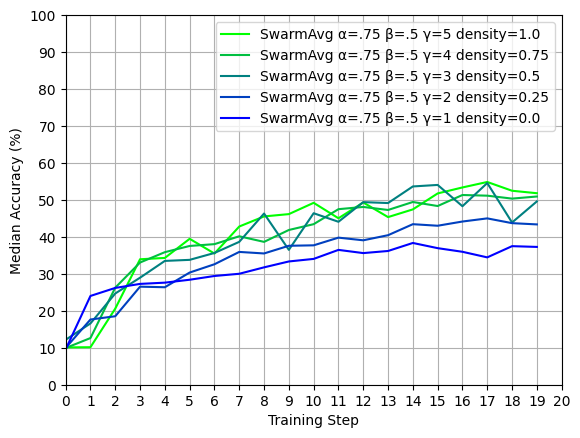
\includegraphics[width=\textwidth]{aeg_sparse_unev_25}
	\caption{Samples=25}
\end{subfigure}
	\caption{Median accuracy by training step across 5 repeats. Quartiles are not shown. Each node has access to a unique set of 3 classes out of 10.}
	\label{aeg9}
\end{figure}


In all three tests, it is clear that a higher density is highly correlated with higher performance in this scenario. It is also noteworthy that with a network density of 0, no matter which volume of data was presented, the accuracy curve was very similar. However, as the density of the network increased, so did the degree at which it was effected by the reduction in data. This scenario also presented graphs with a high degree of noise when compared to other scenarios, despite representing the median of 5 training runs. However, the level of noise is somewhat consistent on all three tests with different data volumes.

	
	\chapter{Critical Evaluation}
	\chapter{Critical Evaluation}
\section{Comparison of SwarmAvg to Other Methods}
Although SwarmAvg has demonstrated promising results, it remains important to conduct a comparative analysis against established methods. This will enable individuals seeking to incorporate distributed machine learning into their future projects to make and informed decisions whether SwarmAvg is the algorithm that they should use.

\subsection{Comparison of SwarmAvg to FedAvg}
SwarmAvg has the significant benefit of being more fault tolerant than FedAvg. This is because FedAvg has a central server, which means that the whole network would stop functioning if the central server is stopped. Not only this, but if a node drops its connection to the server, that node is effectively ignored from training, which has a negative effect on performance. \\

However, SwarmAvg has some significant drawbacks, one of which being that is has been shown to be slower to converge than FedAvg. Not only this, but SwarmAvg can create a significantly higher amount of network traffic than FedAvg or FL in general. This effect is maximised when every node is connected to every other node, meaning that the number of connections scale by $O(n^2)$, where $n$ is the number of nodes. FL will always both number of connections and network traffic scale with $O(n)$, as every node only needs a single connection to the server. However, it is worth noting that SwarmAvg will consume less network traffic in less dense networks of nodes. \\

An important advantage of SwarmAvg over FedAvg is that former can be used in sparsely connected networks without any modification. This means that it is possible for it to SwarmAvg to run even when most nodes in the network are not connected to most other nodes, which may be a more realistic scenario for certain low powered networks of devices such as IoT networks or robotic swarms. For this reason, SwarmAvg may be a better choice than FedAvg for these situations.

\subsection{Comparison of SwarmAvg to SwarmBC}
Despite the fact that this paper did not perform tests on SwarmBC, it is still possible to theoretically compare both SwarmAvg and SwarmBC, based on a comprehensive understanding of the inner workings of each. \\

One of the primary drawbacks of utilizing SwarmAvg as opposed to SwarmBC is the potential occurrence of divergent training during SwarmAvg training. The detrimental effect of divergent training may persist throughout the entire training process, leading to significantly worse performance than anticipated. Several factors can lead to divergent training, with low settings for $\alpha$ and $\gamma$, coupled with a sparsely-connected network, being highly correlated with its occurrence during testing. SwarmBC does not suffer from this issue, as the blockchain ensures that all nodes agree on the same model. However, during testing, divergent training was a rare phenomenon, and its remedy was a simple parameter tuning process upon detection. \\

One drawback of utilizing the SwarmAvg algorithm, as opposed to SwarmBC, is the absence of security features. The utilization of blockchain technology enables the straightforward authentication of nodes utilizing different algorithms that are frequently well-documented and integrated into the blockchain framework. On the other hand, SwarmAvg lacks any built-in authentication mechanism. As a result, to employ it securely, a separate authentication system would need to be implemented to prevent malicious parties from interfering with training. \\

SwarmAvg surpasses SwarmBC in terms of computational efficiency as nodes are not mandated to verify transactions with a blockchain, which involves a comparatively substantial overhead as opposed to simply averaging the models of a nodes neighbours. Consequently, SwarmBC necessitates higher processing power to operate for the same amount of training steps. This overhead could impede the speed of training on a resource-limited system, such as a swarm of drones, as a considerable amount of time is consumed in validating transactions, rather than performing training. Thus, SwarmAvg may be a more fitting choice than SwarmBC for swarms where processing power is a concern.

\section{Evaluation of this Study}
It is of significance to acknowledge that this study presented certain limitations that necessitate careful consideration. The primary concerns are outlined as follows:

\begin{description}
	\item[Small Simulated Number of Nodes: ] A significant concern regarding this study is the limited number of nodes simulated during testing. Several drawbacks of FL in comparison to SL, such as server bottlenecking, are not apparent when testing on a limited number of nodes.
	
	\item[Lack of Testing Overheads: ] In the course of testing the SwarmAvg algorithm, it was determined that the assessment of its performance should be based on training steps rather than time. Although it would have been preferable to evaluate performance in relation to time, this was not feasible due to limitations in resources. The GPUs utilized in this study are primarily optimized for running a single GPU program effectively, whereas this research required multiple nodes to perform training simultaneously. As a result, it was noted during testing that training times varied significantly, rendering time-based measurement impractical due to high levels of noise.
	
	\item[Lack of Simulated Internet Lag: ] The algorithm proposed is designed for usage over the internet. However, the study solely evaluated its performance within a simulated environment, which lacked a time gap between the sending of information from one node to its reception by another. The deliberate omission of this time gap in the simulation aimed to increase the speed of simulations. However, this critical aspect of the algorithm's functionality remains untested as a result.
\end{description}
	
	\chapter{Project Management}
	\section{Time Management}
To assist with planning and organisation of this project, Gantt charts were used. These helped to visualise which tasks needed doing, and also if the project progress was ahead or behind schedule. The Gantt for the interim report can be found in appendix \ref{gc-interim} and the final report Gantt can be found at \ref{gc-final}.

The presented charts represent the final iteration of planning. As described in the following section, changes occurred throughout the project and the Gantt charts were adapted accordingly.

\section{Changing Plans}
At the time of writing the interim report, the project plan was very different to what is presented in this report. Originally, the plan was to implement SL and then to simulate real world problems such as uneven data distribution and sparse networks. However, during the process of implementing the SL algorithm it was apparent that the SL algorithm itself would take a very large amount of time to develop and test. For this reason, the decision was made to refocus the project onto the development of the SL algorithm, and if enough time was available after this, testing a single real world problem may be possible.

Plans were also changed on a smaller scale somewhat regularly. This is due to the experimental nature of this project, and the fact that it was impossible to predict some problems during the planning phase. For example, the parameters $\beta$ and $\gamma$ were not planned for at the start of the project, but whilst experimenting problems arose which seemed like they could be fixed by those parameters. This meant that another implementation had to be created which included those parameters.

\section{Risk Assessment}
The risk assessment was created early on in the project to mitigate any of the major risks. However, none of the described problems arose to an extent which their mitigation plan needed to be followed.
\subsection{Personal Issues}

\subsubsection{Description}
Personal issues which cause the author to be unable to do work, such as illness.

\subsubsection{Risk Calculations}
\emph{Severity (1-5):} 3 \\
\emph{Likelihood (1-5):} 3 \\
\emph{Overall Risk (1-25):} \textbf{9}

\subsubsection{Mitigation}
The codebase will be designed such that individual sections and modules have minimal dependencies on other sections. This means that, even if the author is unable to work for a period of time, some less critical sections can be omitted without significantly impacting the rest of the project.

\subsection{Hardware Failure}
\subsubsection{Description}
Failure on the authors local computer of any kind, such as a graphics card or storage breakage.

\subsubsection{Risk Calculations}
\emph{Severity (1-5):} 4 \\
\emph{Likelihood (1-5):} 2 \\
\emph{Overall Risk (1-25):} \textbf{8}

\subsubsection{Mitigation}
The project will be regularly backed up to GitHub. If a core component of the work computer breaks, the author has access to a personal laptop and the Zepler Labs. The deep learning environment along with dependencies is backed up to the authors Google Drive in the form of a docker image, so that switching to a new computer would be a smooth process.

\subsection{Algorithm Does Not Work Work}
\subsubsection{Description}
The SL algorithm does not function as well as expected.

\subsubsection{Risk Calculations}
\emph{Severity (1-5):} 5 \\
\emph{Likelihood (1-5):} 1 \\
\emph{Overall Risk (1-25):} \textbf{5}

\subsubsection{Mitigation}
It may be possible to shift the project away from SL and onto distributed FL with leader election. FL is more commonly used and therefore has more literature, meaning that it is more likely to be an achievable goal to implement it.
	
	\chapter{Conclusion and Future Work}
	\chapter{Conclusion and Future Work}
\section{Conclusion}
This study has presented a novel SL algorithm algorithm, called SwarmAvg, which enables completely distributed and decentralised machine learning to take place. The algorithm is similar to FL in that it allows each node in the network to hold its own confidential dataset which never needs to be shared with any other nodes.

It has been found that SwarmAvg is less performant than FedAvg in all situations where FedAvg can be applied. However, in many of these scenarios, SwarmAvg reached a similar final accuracy to FedAvg, but training took more iterations to reach this. The area where SwarmAvg showed most potential was when performing training in a sparsely connected network of nodes. This is a situation where FedAvg cannot be used, however SwarmAvg saw only minor reductions in performance when transitioning to this scenario. Unfortunately, it was shown that SwarmAvg performs significantly worse than FedAvg in situations where each node only has access to a small subset of the total classes. Despite the fact that this is an extreme case, unevenly distributed data is an issue for many algorithms in the real world, possibly indicating that SwarmAvg may need further improvements before deployment.

Notwithstanding these disadvantages, SwarmAvg could potentially be a compelling algorithm to employ in particular circumstances. For instance, in a very large swarm, FL may become impossible to use due to the bottleneck of sending all data to a single node, a problem that SwarmAvg does not face. SwarmAvg also may be a better choice if it is known that the network in which the algorithm will be deployed to is very unreliable, with nodes and connections dropping out.

Overall, the goals specified in Section \ref{goals} have been met. Most of the time, SwarmAvg also performed comparably to FedAvg. For these reasons, the author believes this project to be a success.

\section{Future Work}
In the future, a vital step would be to test SwarmAvg on a significantly larger number of nodes, exceeding the current 10 node limit. The aforementioned constraint was established due to limitations on the machine used for training. However, if a data scientist were to design and implement an internet-enabled back-end to the given code, it would be feasible to distribute numerous nodes among multiple training machines, thus enabling the simulation of larger swarms. It would be particularly intriguing to observe the performance of SwarmAvg in scenarios that entail extremely large swarms, but only involve minute amounts of data and transmissions exclusively between a few neighbours for each node who dynamically change over time - a common occurrence in swarm robotics.

A second aspect of future research that could enhance the potential of SwarmAvg involves conducting an in-depth examination of optimal parameters for different situations. For the present study, parameters had to be chosen heuristically to meet testing purposes within the time constraints, potentially resulting in suboptimal outcomes as compared to what could have been achievable.

Merge SL with FL

Dynamic agents

Finally, the scenarios in which SwarmAvg was tested where each node had access to only a subset of the classes left much to be desired. SwarmAvg performed far worse than FedAvg in these situations, however it remains plausible that with future research and modifications, that SwarmAvg may be able to handle these situations better.
	
	\appendix

\chapter{Machine Learning Model} \label{ap:model}
\begin{lstlisting}[language=Python]
inp = Input((28,28))
out = Reshape((28,28,1))(inp)
out = Conv2D(16, (3,3), activation="relu")(out)
out = Conv2D(16, (3,3), activation="relu")(out)
out = Flatten()(out)
out = Dense(256, activation="relu")(out)
out = Dense(128, activation="relu")(out)
out = Dense(10, activation="sigmoid")(out)
model = Model(inputs=inp, outputs=out)
model.compile(
	optimizer="adam",
	loss=SparseCategoricalCrossentropy(),
	metrics=[SparseCategoricalAccuracy()]
)
\end{lstlisting}

\chapter{Gantt Charts}
\newpage
\section{Gantt - Interim} \label{gc-interim}
\begin{center}
	\rotatebox[origin=c]{-90}{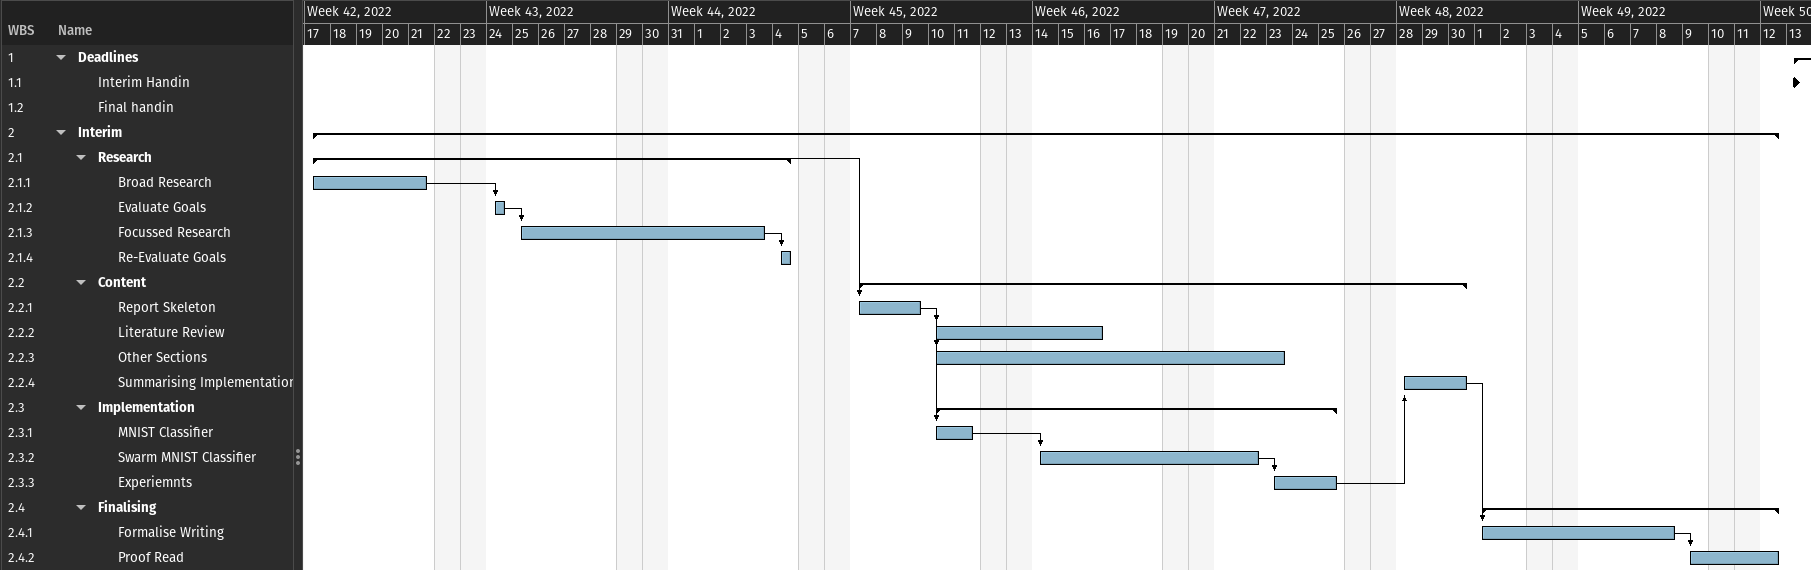
\includegraphics[width=\textheight]{gannt-interim}}
\end{center}

\section{Gantt - Final} \label{gc-final}
\begin{center}
	\rotatebox[origin=c]{-90}{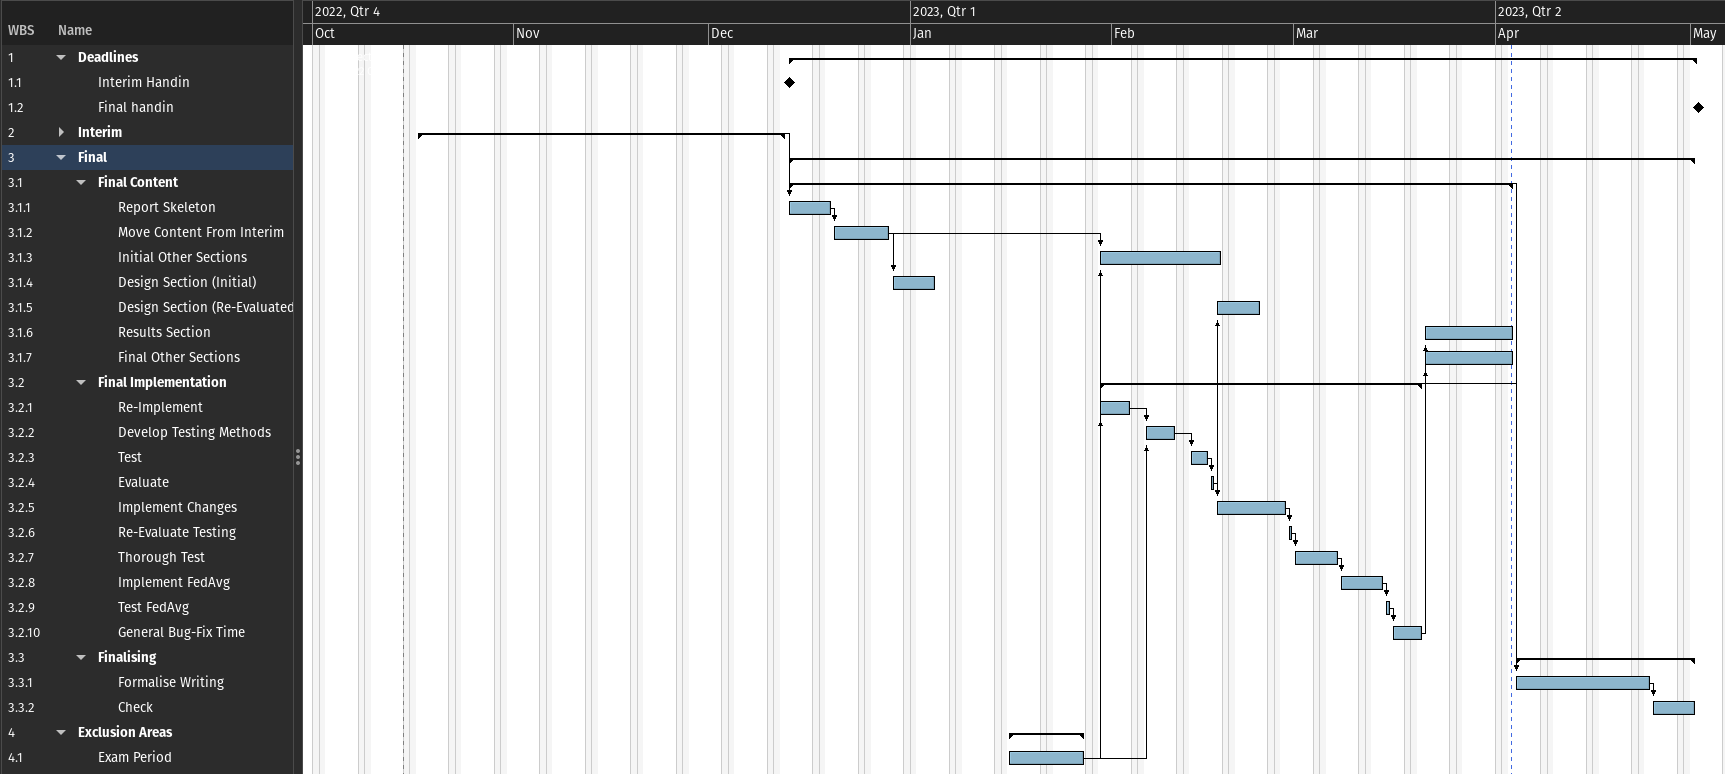
\includegraphics[width=\textheight]{gannt-final}}
\end{center}
	
	\bibliographystyle{ieeetr}
	\bibliography{final}{}
	
\end{document}